\section{Contextualização}
\par
Atualmente a sociedade vive rodeada de tecnologias indispensáveis e de ambientes que se intitulam inteligentes (\textit{smart}), mas nem sempre foi assim.\par
Desde cedo, mesmo antes de existir tecnologia, o homem tendeu a procurar e encontrar coisas que melhorassem a sua vida e bem-estar pessoal e da sociedade, mas para chegar a humanidade está hoje é necessário recuar na história algum tempo para marcos importantes da tecnologia.\par
Um dos marcos muito importantes para o desenvolvimento dos sistemas embebidos e de sistemas de monotorização foi a invenção dos processadores. Com o surgimento dos processadores começaram a surgir os primeiros sistemas embebidos e sistemas de monotorização. Com o passar dos anos até aos dias de hoje a tecnologia tem vindo a evoluir e por consequência os sistemas também se adaptaram para os padrões de atualmente.\par
Uma das partes mais importantes num sistema embebido é a sua interface disponível para o utilizador, as principais e mais usadas nos dias de hoje são a linha de comandos e a WEB, comuns para configurações á distância e as interfaces dos próprios equipamentos como os ecrãs com \textit{software} proprietário.

\section{A Empresa}
\par
A empresa CapTemp, Lda localizada em Pombal, Leiria é uma empresa, focada em desenvolvimento de soluções de monitorização, controlo, supervisão e de soluções à medida consoante os requisitos do cliente. Para criar um sistema de monitorização é necessário o sistema possuir sensores, atuadores, coletores de dados e software para analisar os dados provenientes dos sensores de modo a possuir capacidade de atuar com base nesses valores. A Captemp é responsável pelo desenvolvimento de todos estes componentes passando pelos sensores até ao \textit{software} responsável por analisar e armazenar os dados.\par
Uma das subáreas da empresa é a disponibilização de um registador de temperatura e respetivo \textit{software} certificado para Meteorologia Legal. A Meteorologia Legal é aplicada a todas as câmaras com uma volumetria superior a 10 metros cúbicos, onde a regulamentação indica que tem de existir um sistema certificado para o registo das temperaturas.
Faz parte deste conjunto o \textit{Software} “CapTemp SQL”, representado na figura \ref{figcaptempsql}, responsável por guardar os dados provenientes dos sensores ligados ao registador.\par
\begin{figure}[ht]
  \centering
  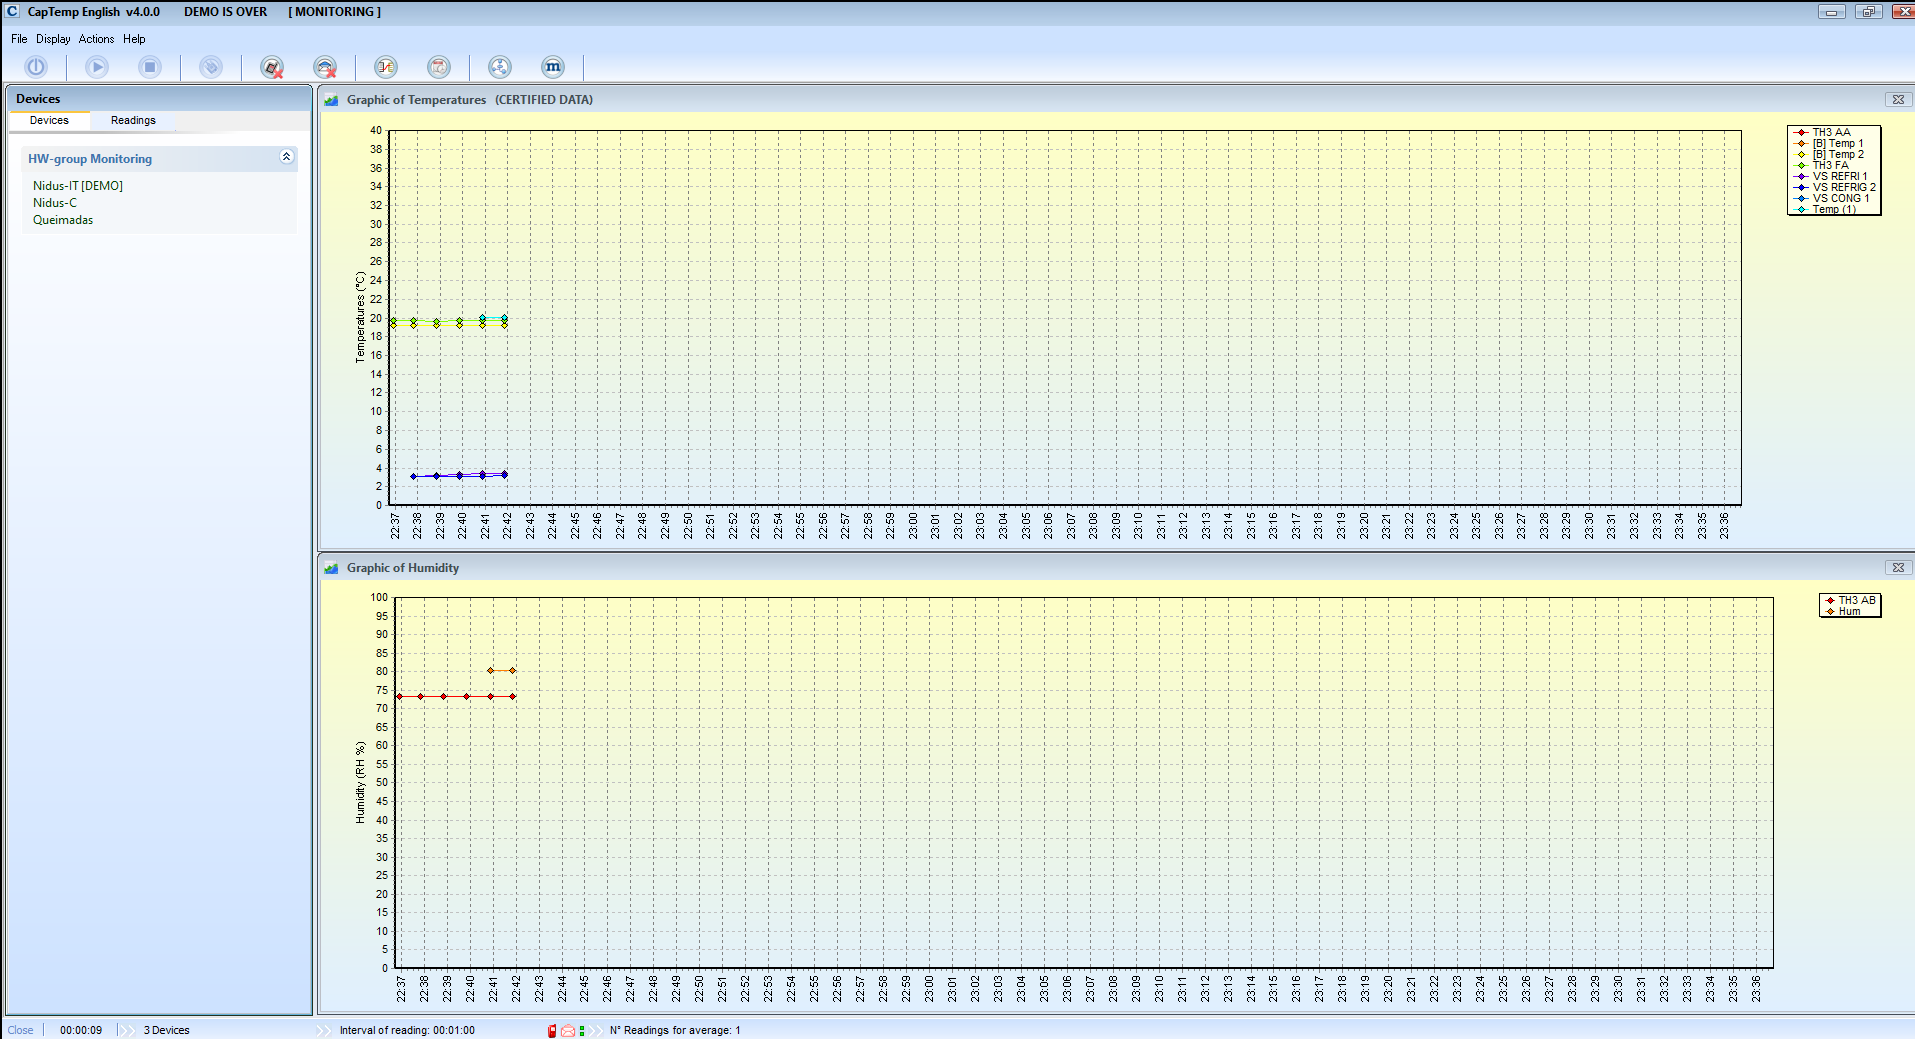
\includegraphics[width=1.00\textwidth]{images/captemp.png}
  \caption{CapTemp SQL}\label{figcaptempsql}
\end{figure}
O registador desenvolvido pela Captemp, representado na figura \ref{fignidusCl} denomina-se por Nidus-C, um registador que suporta até 32 sensores.\par

\begin{figure}[ht]
  \centering
  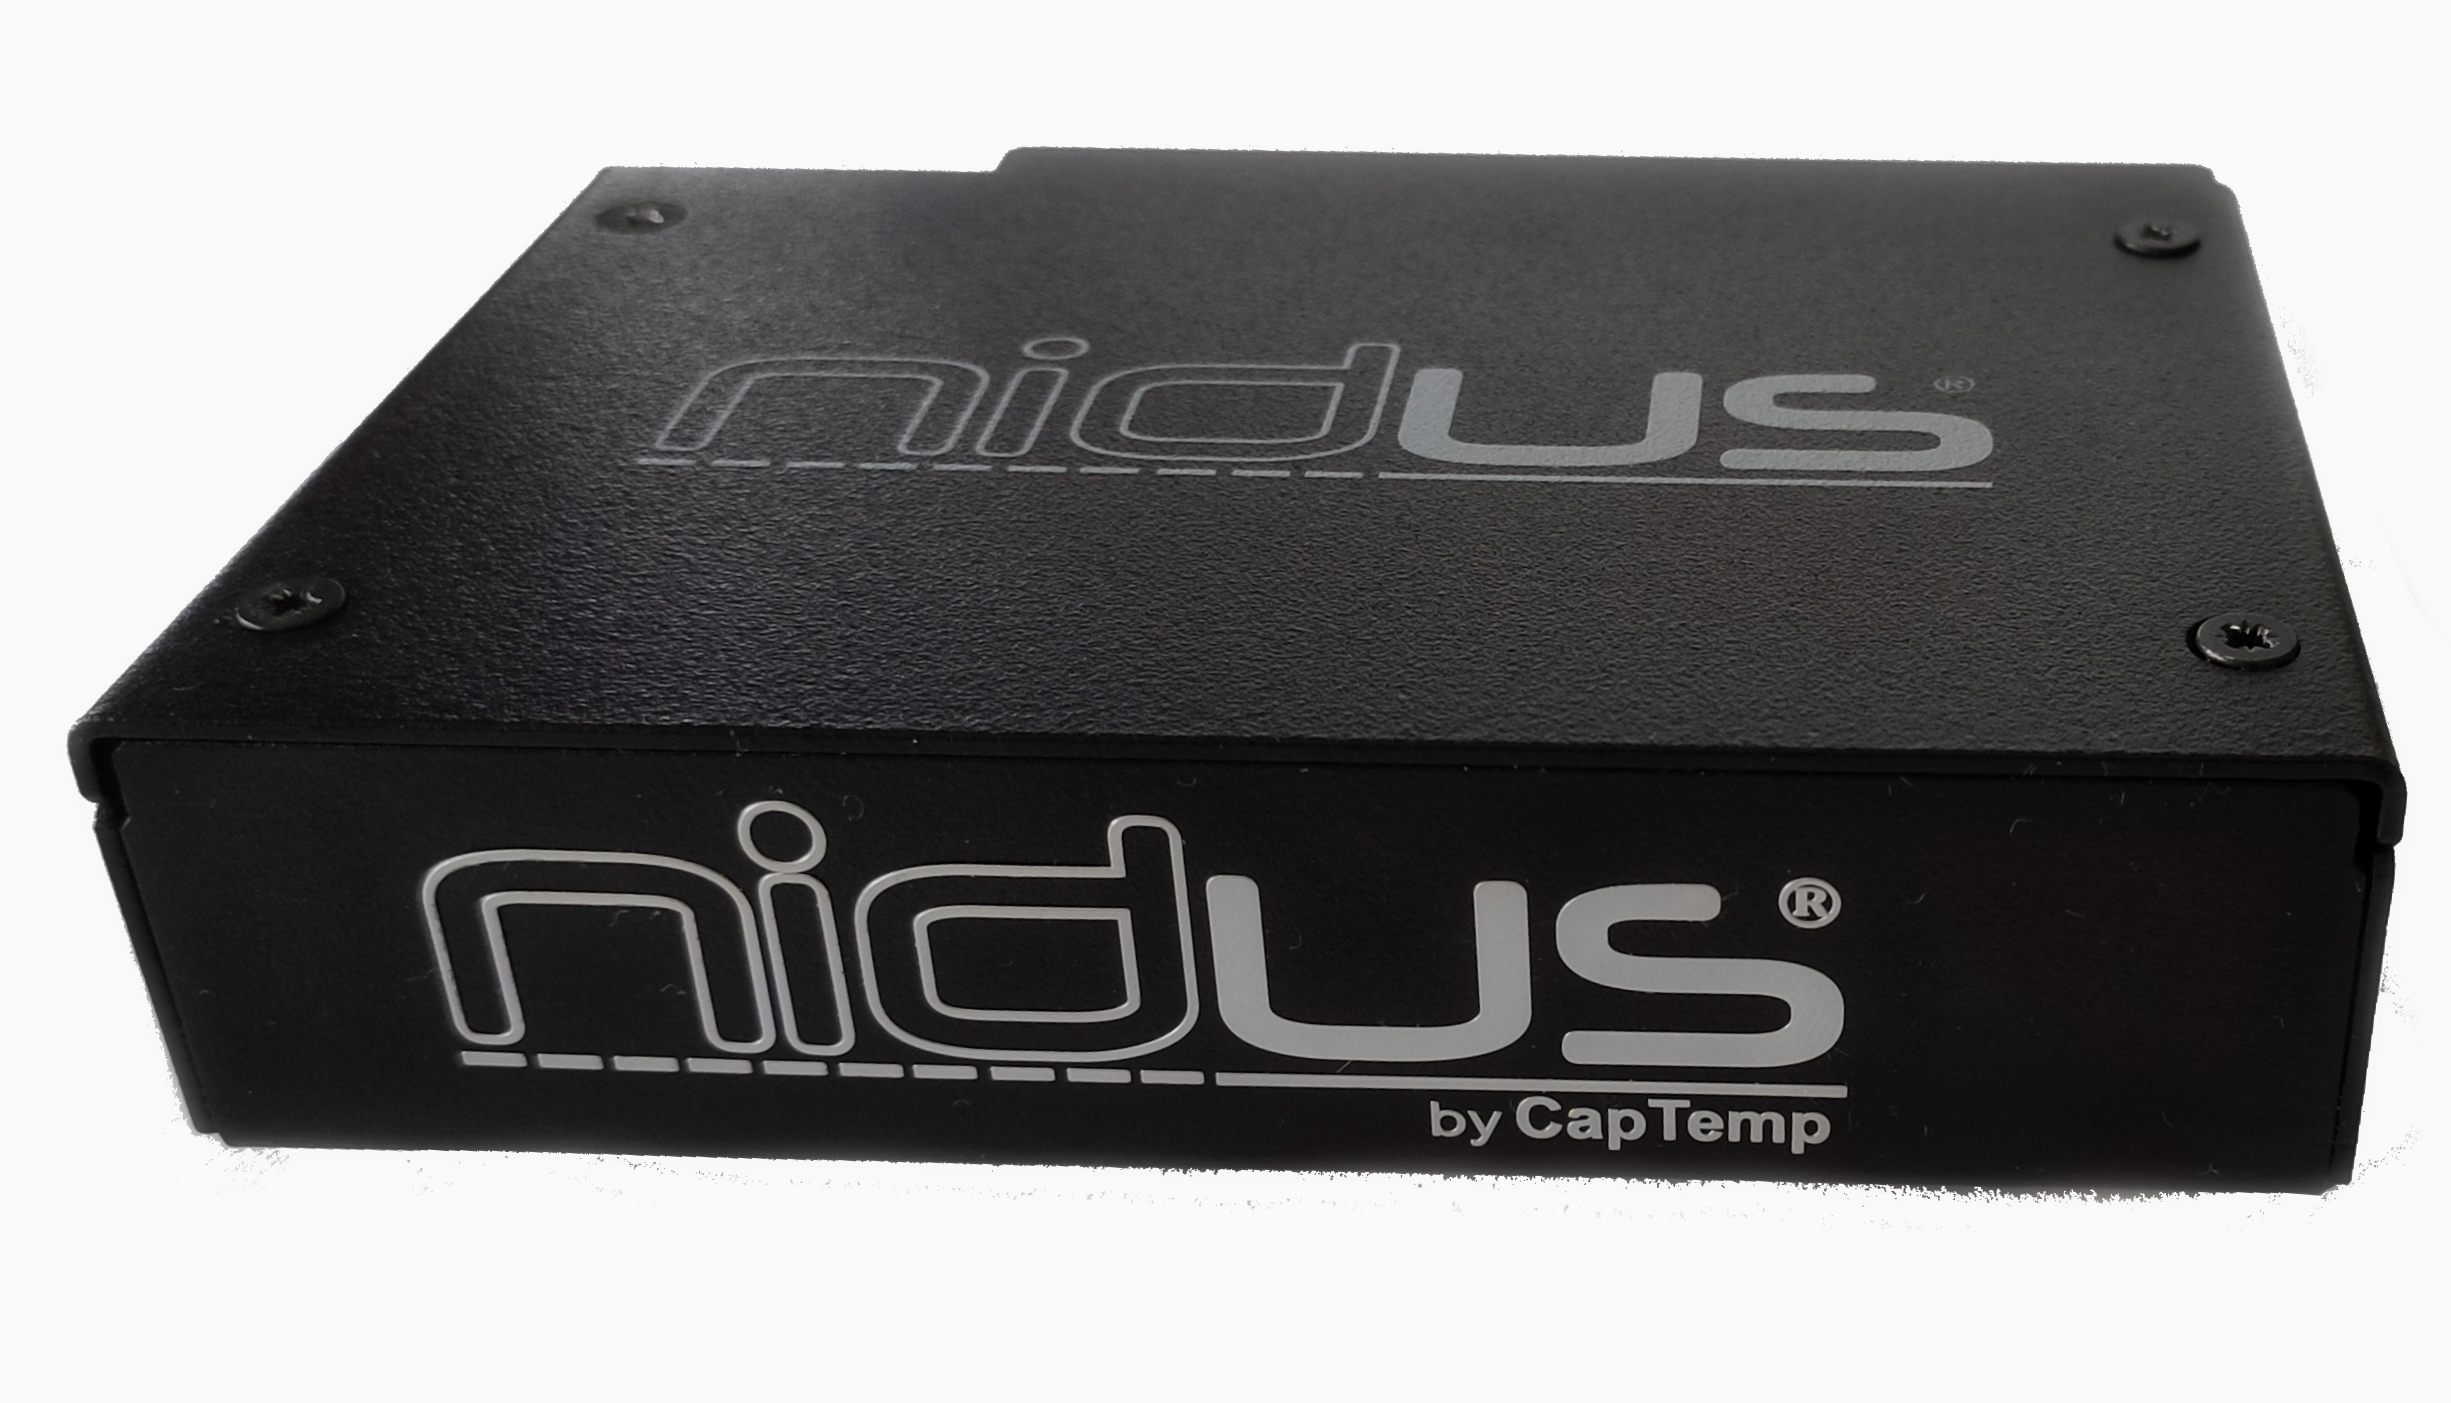
\includegraphics[width=0.45\textwidth]{images/nidus.jpg}
  \caption{Coletor de dados Nidus-C}\label{fignidusCl}
\end{figure}

Com a necessidade de mais funcionalidades, a Captemp criou diversas variantes da Nidus-C, representadas na Figura \ref{fignidusall} para aplicar em outras áreas para além da Meteorologia Legal. Das quais surgiram a Nidus-C+, uma versão similar da Nidus-C acrescentando a possibilidade de adicionar sensores \textit{Wireless}. A Nidus-IT e Nidus-IT+ duas versões com as funcionalidades da Nidus-C e Nidus-C+ respetivamente, acrescentando Inputs e Outputs ao sistema de monitorização. Para soluções exclusivamente \textit{Wireless} nasce a Nidus-W suportando apenas sensores Wireless. Por último é desenvolvido a Nidus-R, baseada na Nidus-IT especialmente desenhada a pensar em ambientes IT com suporte para montagem em bastidores.
\par
\begin{figure}[ht]
  \centering
  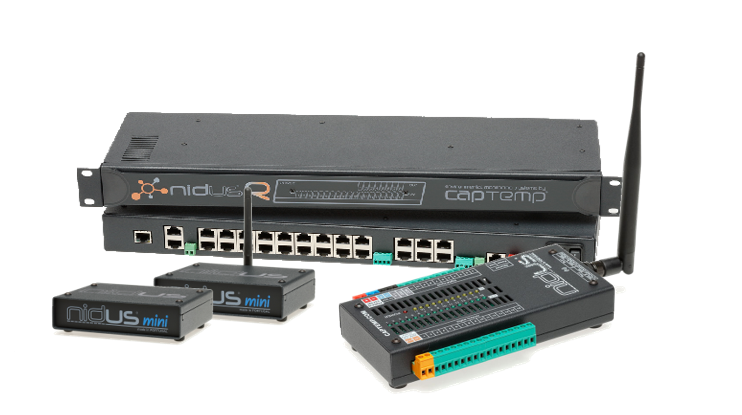
\includegraphics[width=0.65\textwidth]{images/nidusall.png}
  \caption{Universo Nidus}\label{fignidusall}
\end{figure}

No setor dos sensores foi desenvolvido o TH3, um conversor RS485 permitindo às diversas Nidus, ligar por RS485 a sensores 1Wire além dos dois inputs possuídos no TH3. Nos sensores \textit{Wireless}, foi desenvolvido o Airo à semelhança do TH3 possui dois inputs, um ecrã e possibilita a ligação de sensores 1Wire. Permite ainda a leitura de todos os Airo adicionados na Nidus ao mesmo tempo, tecnologia desenvolvida pela Captemp denominada por Captemp AST \cite{Captemp_AST}. Ambos os sensores estão representados na Figura \ref{figairoth3} 
\begin{figure}[ht]
  \centering
  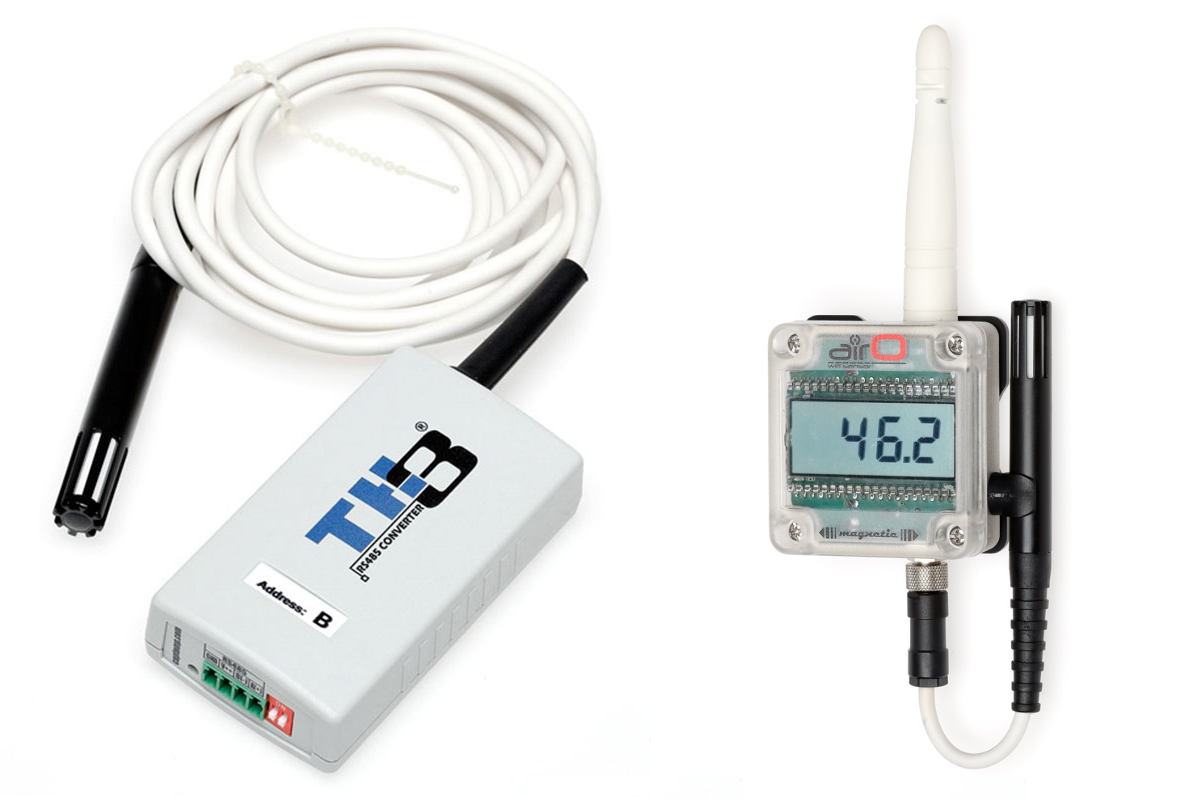
\includegraphics[width=0.45\textwidth]{images/th3airo.png}
  \caption{ TH3 e Airo}\label{figairoth3}
\end{figure}
\par
Em desenvolvimento encontram-se sensores com recurso a tecnologias NB-Iot, \textit{beacons} BLE e Lora entre outras soluções tais como sistemas de rastreamento de Febre em tempo real com recurso a inteligência artificial.
\par
A Captemp desenvolve igualmente um portal \textit{Cloud} denominado Senslive (Figura \ref{figsenslive}) que possibilita a centralização dos sistemas de monitorização numa única plataforma \textit{Cloud}.

\begin{figure}[ht]
  \centering
  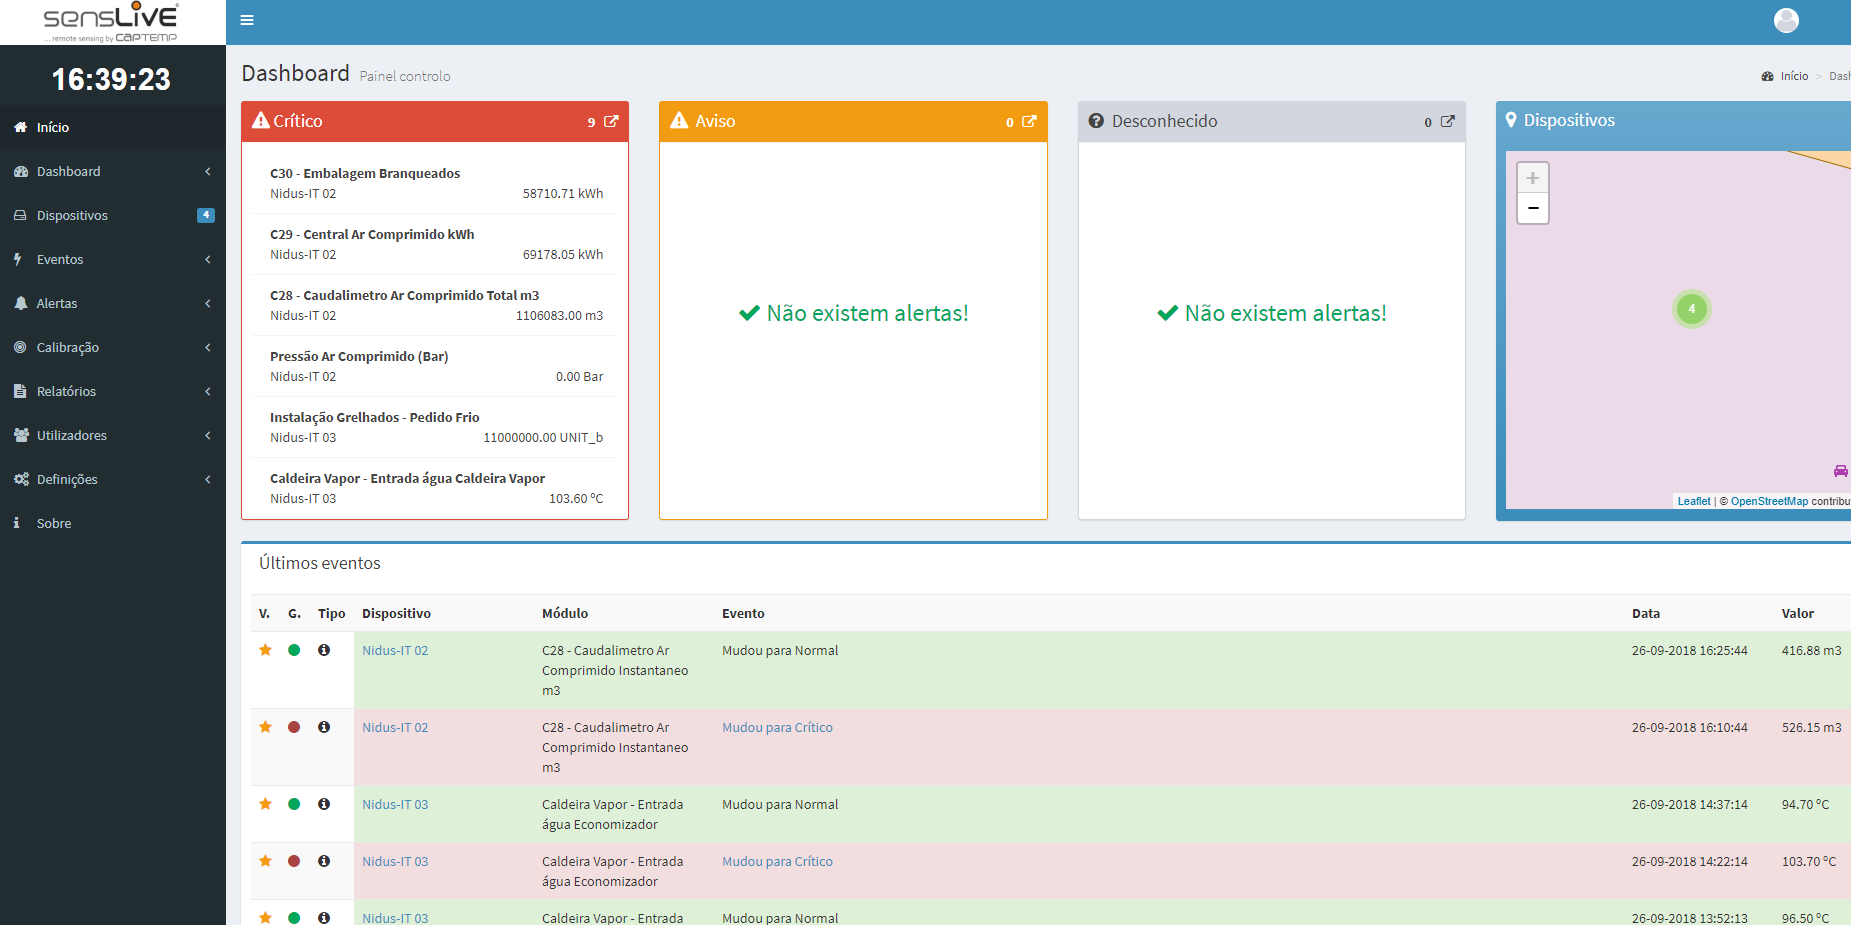
\includegraphics[width=0.95\textwidth]{images/mwsnap0791.png}
  \caption{ Portal Senslive}\label{figsenslive}
\end{figure}



\section{Motivação e Objetivos}
\par
O estágio é uma forma do estudante colocar numa situação de contexto profissional os conceitos adquiridos em contexto académico. A realização de um estágio é também uma mais valia pois possibilita o adquirir de experiência profissional que não é possível obter em contexto escolar.
\par
A Captemp com os projetos a desenvolver pretende melhorar constantemente os seus equipamentos e as suas interfaces, por questões de \textit{Markting} quer pelo próprio evoluir da tecnologia e necessidade de novas funcionalidades e o seu desenvolvimento requer o alojamento de mais recursos como por exemplo a memória ou disco, estes limitados nestes tipos de equipamentos e onde é preciso fazer uma correta escolha de soluções e de implementação. 
\par
Ao longo do estágio, o objetivo será estudar variados mecanismos que permitam adotar recursos web modernos nos equipamentos de baixos recursos. Serão aplicados vários conhecimentos adquiridos durante o percurso académico de modo a melhorar a interface para o utilizador, técnicas de otimização de código, compressão de ficheiros, manipulação de imagens de modo a ocupar o mínimo de espaço permitindo futuros desenvolvimento e melhorias, dando continuidade ao suporte do projeto Nidus. Igualmente serão criados três novos projetos de desenvolvimento de novos equipamentos e soluções que tiram partido de novas tecnologias como o NB-Iot e \textit{beacons} BLE onde é necessário devido á escassez de recursos fazer a correta gestão dos mesmos e a implementação de variados algoritmos.
\par
Nas seguintes secções são apresentadas uma breve descrição de cada projeto, dos equipamentos já existente e desenvolvido, e as funcionalidades a desenvolver em cada projeto.
\subsection{Nidus}
\par
O projeto "Nidus" tem como objetivo dar suporte ao \textit{Front-end} das Nidus já existentes para correções de bugs encontrados em versões anteriores, otimização de código, de modo a ocupar o mínimo espaço, possibilitando deixar memória livre para desenvolvimentos futuros, desenvolver versões customizadas com \textit{layouts} a pedido do cliente com funcionalidades especificas, ou simplesmente melhorar a página seguindo a tendência de equipamentos concorrentes.
\subsection{NB-Iot}
Com o surgimento da nova tecnologia NB-Iot surgiu a necessidade de serem criados equipamentos que tirem partido dessa tecnologia e as suas vantagens. Para tal durante o estágio será desenvolvido um dos equipamentos que tira partido da tecnologia. Este projeto tem como por objetivo criar uma versão de raiz, simplificada e mais barata de um outro equipamento de NB-Iot em desenvolvimento pela Captemp, através do módulo Xbee da DIGI e da sua programação em Micropython. Durante o projeto será necessário garantir a correta gestão de memória, gestão de Logs internos, comunicação com os sensores físicos, comunicação bidirecional e encriptação com o portal Senslive.
\subsection{Kea Tracker}
O "Kea Tracker" é um projeto de \textit{beacons} BLE que comunicam com o \textit{smartphone}, onde é possível definir alertas locais no \textit{smartphone} e envio dos dados obtidos dos sensores dos \textit{beacons} e envio para a plataforma Senslive.
Tal como o projeto anterior será necessário além de criar uma aplicação para \textit{smartphone}, criar \textit{Firmware} específico para os \textit{beacons} que na ausência de comunicação com o \textit{smartphone} devem armazenar em Log as leituras dos sensores e quando este está ao alcance descarregar para o \textit{smartphone}.
\subsection{dot.Tracker}
A pedido de um cliente foi solicitado o desenvolvimento de uma plataforma para localização de pessoas e objetos em ambientes \textit{indoor}. O cliente pretende ter uma plataforma onde seja capaz de ver em tempo real a posição de pessoas e objetos definidos previamente, definir zonas de alerta, e consultar o histórico de movimentos. Neste projeto irão ser usados \textit{beacons} BLE e vários \textit{Gateways} BLE estrategicamente colocados no edifício e responsáveis por receber o \textit{broadcast} dos \textit{beacons} que por sua vez transmitem para o servidor através da rede informática do cliente do serviço. O projeto é constituído pelo desenvolvimento da plataforma de gestão e visualização, pelo recetor dos pacotes provenientes dos equipamentos e respetivos cálculos segundo o algoritmo a adotar.

\section{Problemas identificados}
Foram identificados diversos problemas em cada um dos projetos a desenvolver durante o estágio. Uma breve descrição é apresentada de seguida.
\par
A página WEB da Nidus desde a sua criação já sofreu muitas alterações para seguir os padrões e tendências da concorrência e, portanto, está em constante atualização. Atualmente com a mundialização quase todas as pessoas sabem inglês, mas existem algumas pessoas que ou não sabem ou preferem usar a língua nativa. Para tal a Captemp pretende desenvolver uma página WEB com um sistema de tradução e diversas línguas que seja possível de alojar na memória do equipamento, devido aos problemas já referidos para o utilizador escolher a linguagem e assim cativar mais clientes e expandir a Captemp para outros países. Com o acréscimo do serviço de internalização surge o problema de uma interface com necessidade de mais armazenamento. Terão de ser estudadas otimizações que se possam implementar no código já existente. Existe a necessidade de estudar o melhor método de compressão da página mantendo o GZIP utilizado atualmente ou migrar para outro mais recente como o Brotli e a compressão de imagens migrando as imagens existentes para imagens SVG, possibilitando outras soluções para a página com sistemas mais interativos e ocupando o menor espaço disponível. Além dos problemas referidos anteriormente poderão surgir novas funcionalidades, a pedido de clientes, como por exemplo páginas com layout específicos ou novos sensores e a simples correção de possíveis Bugs encontrados.
\par
Outro problema a resolver detetado pelo \textit{feedback} recebido dos clientes é a complexidade para a criação de eventos, ações e reações, que controlam o Sistema Nidus. Para isso a Captemp pretende reformular a estrutura de gestão de eventos para um sistema mais visual e atual similar ao Scratch, um \textit{software} utilizado atualmente para ensinar a crianças as bases da programação e elas mesmos criarem alguns programas sem saber nenhuma linguagem de programação. Na figura \ref{scratch} é apresentado um exemplo de programação usando a ferramenta Scratch, onde o utilizador com um sistema de blocos pode criar condições e eventos a despoletar consoante algumas condições.

\begin{figure}[ht]
  \centering
  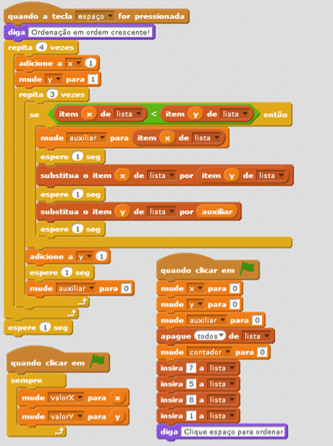
\includegraphics[width=0.50\textwidth]{images/scratch.png}
  \caption{ Programação com a ferramenta Scratch}\label{scratch}
\end{figure}

\par Outros problemas existentes, a resolver durante o estágio, são a criação de sistemas \textit{low-cost}, de outros equipamentos CapTemp, para clientes que não necessitem de tantas funcionalidades com a introdução da alternativa para NB-Iot com recurso ao módulo Xbee da Digi, e a substituição de produtos antigos descontinuados, os data-logger(Figura \ref{ds1921}) e sua substituição por similares com as mesmas funções e mais tipos de sensores disponíveis, uma necessidade também já requisitada pelos clientes que pretendem monitorizar mais grandezas além da temperatura, mas com os padrões e tecnologias dos dias de hoje e com suporte para o novo Portal da Captemp o Senslive. Ou simplesmente o desenvolvimento de novos produtos a pedido dos clientes.

\begin{figure}[htb]
  \centering
  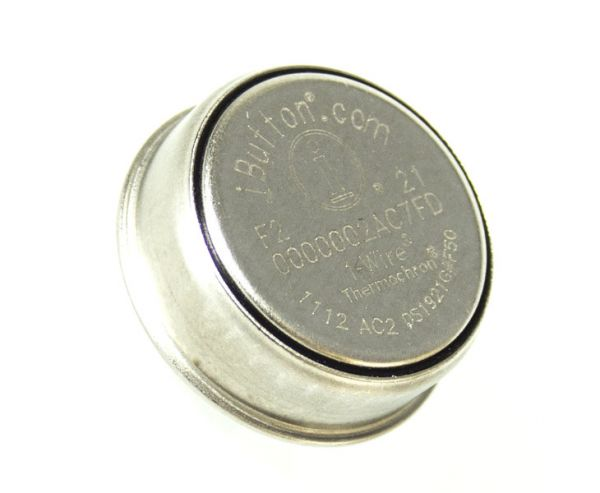
\includegraphics[width=0.20\textwidth]{images/ds1921.jpg}
  \caption{Data Logger iButton}\label{ds1921}
\end{figure}


\par
Em resumo os problemas a solucionar durante o estágio podem ser encontrados na seguinte lista:
\begin{itemize}
\item Melhorar a compressão da página WEB da Nidus;
\item Melhorar a compressão das imagens presentes na página WEB da Nidus;
\item Correção de Bugs da página Web da Nidus;
\item Melhorar o processo de criação de eventos;
\item Criação de uma página com sistema de tradução automático;
\item Versões customizadas da página WEB a pedido do cliente;
\item Seguir as tendências da concorrência;
\item Criação de soluções/equipamentos de baixo custo;
\item Substituição de produtos descontinuados;
\item Desenvolvimento de produtos à medida do cliente.

\end{itemize}

\section{Organização do relatório}

\par Este presente relatório está dividido em 5 capítulos. O primeiro capítulo faz a introdução ao tema e é apresentado os objetivos, o enquadramento do estágio e alguns aspetos inicias a considerar. 
\par No capítulo seguinte é apresentada a tecnologia e hardware pesquisado com fim a dar suporte a este mesmo estágio e uma pequena pesquisa sobre projetos/produtos similares quer na finalidade quer nas tecnologias usadas e o estado atual de cada projeto. 
\par O capítulo 3 apresenta o trabalho desenvolvido durante o estágio na empresa para a resolução dos problemas identificados. Este capítulo apresenta os detalhes técnicos das soluções escolhidas. 
\par No capítulo 4 são descritos os resultados dos testes efetuados às soluções propostas e desenvolvidas no capítulo 3.
\par Por fim no capítulo 5 é apresentada uma breve conclusão de todo o trabalho, dificuldades e algumas sugestões para futuras implementações. 

